%
% Spark reference architectures
% Copyright (C) 2016 Martin Zapletal
%
% This program is free software: you can redistribute it and/or modify
% it under the terms of the GNU General Public License as published by
% the Free Software Foundation, either version 3 of the License, or
% (at your option) any later version.
%
% This program is distributed in the hope that it will be useful,
% but WITHOUT ANY WARRANTY; without even the implied warranty of
% MERCHANTABILITY or FITNESS FOR A PARTICULAR PURPOSE.  See the
% GNU General Public License for more details.
%
% You should have received a copy of the GNU General Public License
% along with this program.  If not, see <http://www.gnu.org/licenses/>.
%

\documentclass[a4paper, 10 pt, conference]{IEEEtran}

\usepackage{graphicx}
\usepackage{interval}
\usepackage{listings}
\usepackage{hyperref}
\usepackage{siunitx}
\usepackage{amsmath}

\sisetup{load-configurations = abbreviations, binary-units = true}
\intervalconfig {
soft open fences ,
separator symbol =; ,
}

\title{Spark Reference Architecture \\ Financial transactions streaming}

\author{Martin Zapletal%$^{1}$% <-this % stops a space
%\thanks{Supported by Cake Solutions Limited}% <-this % stops a space
%\thanks{$^{1}$Martin Zapletal is the CTO at Cake Solutions Inc., 195 Plymout Street, 11201, New York {\tt\small martinz at cakesolutions.net}}%
}


\begin{document}

\maketitle
\thispagestyle{empty}
\pagestyle{empty}

%%%%%%%%%%%%%%%%%%%%%%%%%%%%%%%%%%%%%%%%%%%%%%%%%%%%%%%%%%%%%%%%%%%%%%%%%%%%%%%%
\begin{abstract}

TODO

\end{abstract}


%%%%%%%%%%%%%%%%%%%%%%%%%%%%%%%%%%%%%%%%%%%%%%%%%%%%%%%%%%%%%%%%%%%%%%%%%%%%%%%%
\section{Introduction}

TODO

\section{Reference implementation}

This architecture was used in a financial transaction processing system. The system continuously receives data from either a streaming integration point or files, processes and transforms the data, validates them against known records and finally stores the results.

The application receives multiple types of inputs. One are files from other financial institution containing a set of transactions. The other one is integration with other systems through Apache Kafka. The records are processed, validated against known data stored in Cassandra database, transformed and finally stored in Cassandra and relevant information sent to integration points with other internal systems. The application has strict requirements for uptime, availability, consistency, data integrity, scalability and cost optimisation while ideally using OS technologies. For those reasons Mesosphere DSOS was chosen for infrastructure automation, cluster and resource management.

\section{Main components}

The main components in this architecture are data sources (file source and Apache Kafka), stream processing pipeline and database. High level architecture is displayed on figure~\ref{fig:components}. 

\begin{figure}[hb]
	\begin{center}
		\caption{Components}
		\label{fig:components}
		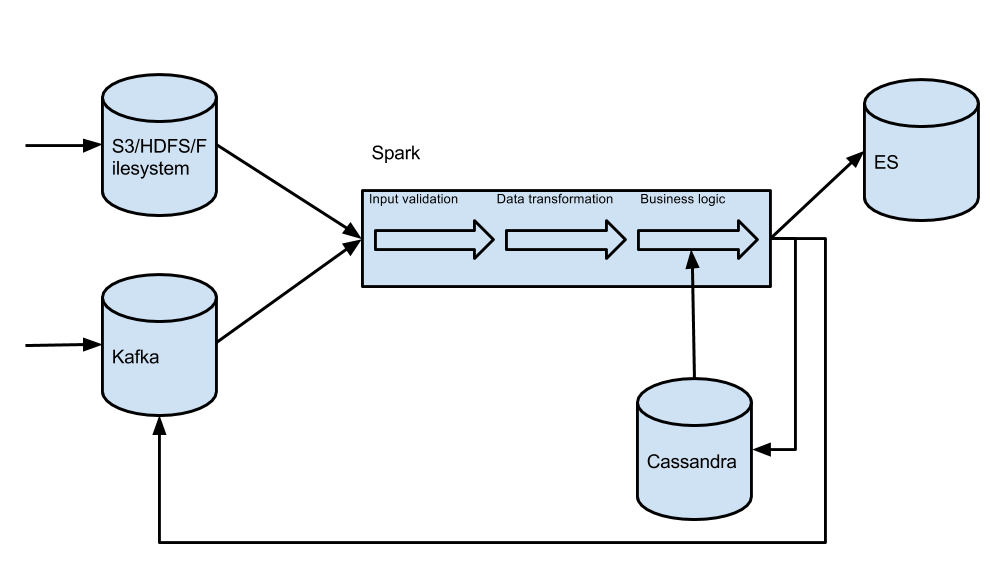
\includegraphics[width=7cm,keepaspectratio]{architecture-diagram.png}
	\end{center}
\end{figure}

\subsection{Data sources}
In this reference architecture two different data sources are used. An input directory is used for historical reasons as an integration point between financial institutions. A file in a known format is uploaded to the directory in defined intervals. Apache Spark file stream source can monitor a directory and process each new file as it is added to the directory.
Apache Kafka is used for integration with other internal systems. Kafka is a distributed log often used for integration for its scalability, reliability, durability, replayability and other attributes. Spark provides a Kafka input stream and its direct version as options to stream data from Kafka.

\subsection{Stream processing}
After ingesting data from the sources they need to go through a processing pipeline with guarantees satisfying the requirements. The requirements and guarantees provided by Spark are in detail described in next section.
The stream processing pipeline is used for the following purposes.

\subsubsection{Input cleaning and validation}
The inputs are validated. For example the input may not be in the correct format, expected schema invalid, required fields may be missing, outliers may be checked, input data from different publishers standardised and cleaned or other validation done and data filtered.

\subsubsection{Data transformation}
Before processing the data we may need to transform the data into correct format. That may involve transforming from XML/json/cvs/binary or other data format to business logic representation that is easier and safer to work with, query and analyse.

\subsubsection{Business logic implementation}
After the data are in correct format for processing we can apply the actual business logic rules. It may involve queries, real time analytics, aggregations, training and application of machine learning model or asynchronous communication with other systems. In this particular architecture the input data are validated and enriched using records stored in Cassandra database.

\subsubsection{Data storage}
The processed data are stored in a database solution. Firstly, the business logic records are updated using the previously applied business rules. Secondly, an analytics data store is updated with the new records for advanced analytics and search purposes. 

\subsubsection{Result integration}
Enterprise systems are often large distributed application consisting of many services, independent applications and modules. Spark is used to provide updates about the real time processing to the interested services by publishing a stream to Apache Kafka. Kafka is then used as streaming data platform for other systems to subscribe to real time updates with Kafka's strong guarantees.

\section{Streaming data platform}

\begin{figure}[hb]
	\begin{center}
		\caption{Streaming data platform}
		\label{fig:streamingDataPlatform}
		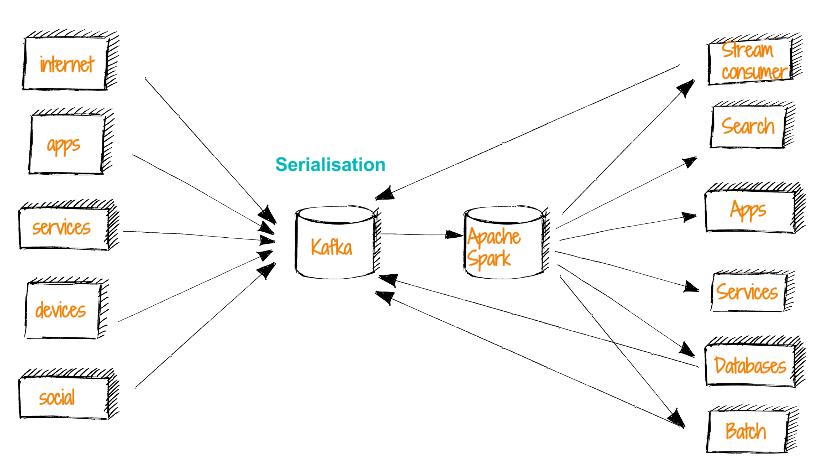
\includegraphics[width=7cm,keepaspectratio]{streaming-data-platform.png}
	\end{center}
\end{figure}

Commonly, ETL and data processing was done in batches and batch processing architectures, supported by Hadoop and similar technologies was common. Due to lack of flexibility and often slow results Lambda Architecture was introduced. It uses batch layer to still deliver correct result and streaming layer to deliver some or partial results quickly.
ETL and batch processes were still often run in intervals capturing a current snapshot of the data to mimic streaming, often due to insufficient access to streaming solutions. The approaches to data processing were questioned with the introduction of Streaming data platform (sometimes called Kappa architecture) in [https://www.oreilly.com/ideas/questioning-the-lambda-architecture] displayed on figure~\ref{fig:streamingDataPlatform}.

This architecture uses a solution that can handle large scale streaming data such as Apache Kafka. Any team, application, system, service, sensors, devices etc. can publish their data into the streaming platform. On the consumer side anyone can subscribe to the streaming data platform and consume the streams they are interested in. They are kept up to date with the latest data using a streaming solution and depend on guarantees a particular streaming solution offers.
The advantages compared to batch processing are obvious. Not only are the same guarantees of batch processing maintained, but the consumers are kept up to date in near real time.
Apache Spark Streaming module fits very well into such architecture with reliable delivery, fault tolerance, throughput, scalability and integration with many other streaming solutions. It is used as a consumer and for transformation, repartitioning of data and preparation for the subscribers to use efficiently as displayed on figure~\ref{fig:streamingDataPlatform}.

\section{Requirements and Spark's guarantees}

\subsection{Data consistency}

\subsection{Delivery guarantees}

\subsection{Fault tolerance}

\subsection{Order}
Ordering
Event time processing

\subsection{Scalability}
Elasticity
Dynamic
Dynamic changes to pipeline

\subsection{Latency and throughput}

\subsection{Serialisation and versioning}

\section{Alternatives and competitors}

\section{Conclusion}











The sensors shown here as consumer-grade wearables perform only the basic hardware interaction: there is no pre-processing of the recorded data. The system accepts accelerometer, gyroscope, heart rate and---where available---data from strain gauges in smart clothes. The mobile application performs the real-time processing of the inputs, displays the next exercise the user should perform (allowing the user to change the suggestion by simply walking to a station for a different exercise, or by beginning a different exercise). The mobile application also prompts the user to confirm correct labels for the recorded data. \emph{This is the key component in the entire system: the frictionless user experience gives the system very accurate labels on very clean data}.

The mobile submits the entire session data (the sensor data, matching labels and latest user behaviour models) in a single request to the Akka \cite{akka} cluster---a CQRS/ES \cite{cqrs-es} microservice implementation. The Akka cluster stores its events and snapshots in a journal, implemented by the Apache Cassandra \cite{apache-cassandra} database. Alongside the events and snapshots, which are opaque to non-Akka systems, the \texttt{exercise} microservice saves the sensor data and the matching labels in a properly formed tabular structure. This structure allows the Apache Spark \cite{apache-spark} cluster to be used for typical big data tasks.

The Spark cluster Lorem ipsum dolor sit amet, consectetur adipiscing elit. Donec magna purus, gravida et molestie a, bibendum et libero. Maecenas sed egestas erat. Suspendisse ullamcorper posuere erat, et finibus turpis tempor varius. Aenean tempus tellus sit amet arcu interdum, eu ornare nulla egestas. Nulla facilisi. Sed imperdiet urna et convallis consequat. Nullam nec ex eu leo auctor interdum eu id nunc. Fusce fermentum tempor gravida. Morbi sit amet augue a erat condimentum vulputate. Proin sed mattis lorem, viverra condimentum metus. Suspendisse luctus aliquam placerat. Donec sit amet mollis massa. Aliquam luctus dui in imperdiet accumsan. Nam nisi ligula, dapibus id interdum in, dictum efficitur ligula. Donec bibendum mollis convallis. Fusce maximus non orci quis laoreet.

The models are implemented in Lorem ipsum dolor sit amet, consectetur adipiscing elit. Donec magna purus, gravida et molestie a, bibendum et libero. Maecenas sed egestas erat. Suspendisse ullamcorper posuere erat, et finibus turpis tempor varius. Aenean tempus tellus sit amet arcu interdum, eu ornare nulla egestas. Nulla facilisi. Sed imperdiet urna et convallis consequat. Nullam nec ex eu leo auctor interdum eu id nunc. Fusce fermentum tempor gravida. Morbi sit amet augue a erat condimentum vulputate. Proin sed mattis lorem, viverra condimentum metus. Suspendisse luctus aliquam placerat. Donec sit amet mollis massa. Aliquam luctus dui in imperdiet accumsan. Nam nisi ligula, dapibus id interdum in, dictum efficitur ligula. Donec bibendum mollis convallis. Fusce maximus non orci quis laoreet.

\subsection{Mobile application}

The sensors send the data in \SI{1}{\second} batches; the application on the mobile resamples the sampling rate to \SI{50}\hertz. (Accelerometer and gyroscope typically sample at this rate, heart rate and the strain gauges in smart clothes can be up-sampled to \SI{50}{\hertz} easily.) The mobile application ingests the data from the sensors and, together with a statistical model of the user's short-term behaviour, attempts to identify the movement. The models in the mobile application can make successful predictions of sequence of exercises in a session and the properties of each exercise (i.e. weight, number of repetitions, duration, intensity). The model used to predict sequence of exercise sessions and exercises within a session is a Markov chain \cite{markov-chain-exercise}. This approach allows the application to deal with the reality of exercise in a public gym, where the station for the next suggested exercise might not be available. The Markov chain, together with a bio-mechanical model of the main muscle groups, gives the users the flexibility to achieve their workout targets even in crowded gyms. The sequence of exercise predictions for one particular exercise sessions are illustrated on \autoref{fig:model-sequence}.

\begin{figure}[h]
	\begin{center}
		\caption{Exercise sequence model}
		\label{fig:model-sequence}
		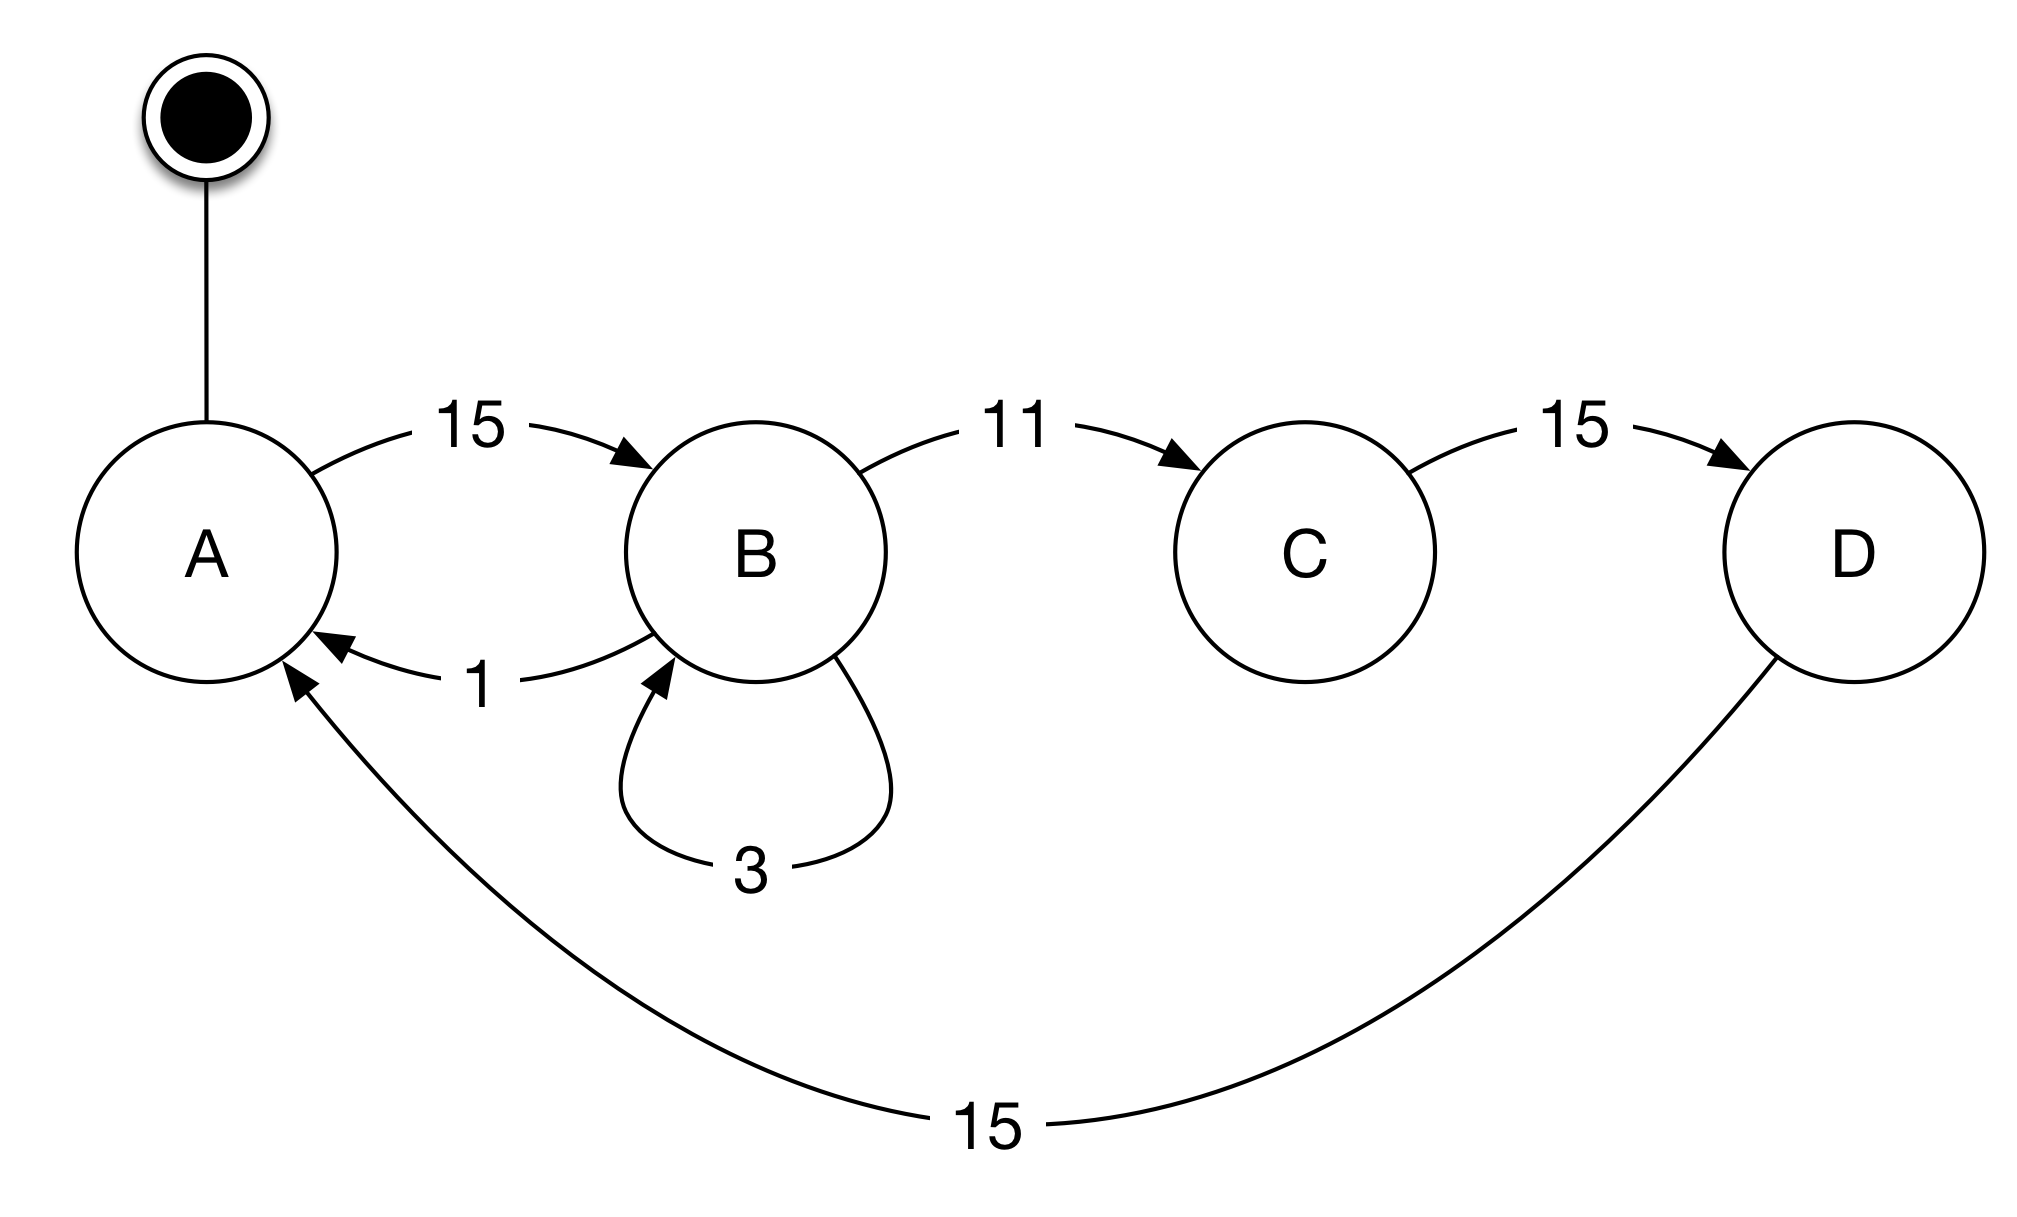
\includegraphics[width=7cm,keepaspectratio]{ri-model-sequence.png}
	\end{center}
\end{figure}

The numbers in \autoref{fig:model-sequence} represent the count of transitions taken; hence it is possible to calculate the probability of transition from any given state. The state names represent the exercise labels, in real application, they are the real exercise names. The mobile application can either receive the chain when the user selects one of the pre-defined exercise programmes, or it can construct the chain from empty if the user choses to start his or her custom workout. This gives the application an intuitive feel; its suggestions are what the users usually do. Finally, the information in the chain allows the system to identify the most popular sequences of exercises, to identify exercises that the users do not like; more interestingly, the system can use the information in the chain to identify sequence of exercises that leads to the best improvement. (At this point, we do not define what the improvement is: in some applications, it may be weight loss; in other applications, it may be greatest mobility range improvement; and many others.)

To make the next-exercise prediction more accurate, the mobile application uses fined-grained location services. The location services are implemented using bluetooth beacons. The beacons operate in the iBeacon mode \cite{ibeacon}; each beacon in this mode transmits its identifier, a major, and minor values. The mobile application sets up continuous scanning of a major value which identifies exercise equipment, receiving notifications of beacons and their minor values as they come into range. The mobile application then filters the exercise states keeping only those that are associated with a particular area. (Viz \autoref{fig:model-sequence+location}.)

\begin{figure}[h]
	\begin{center}
		\caption{Exercise sequence model}
		\label{fig:model-sequence+location}
		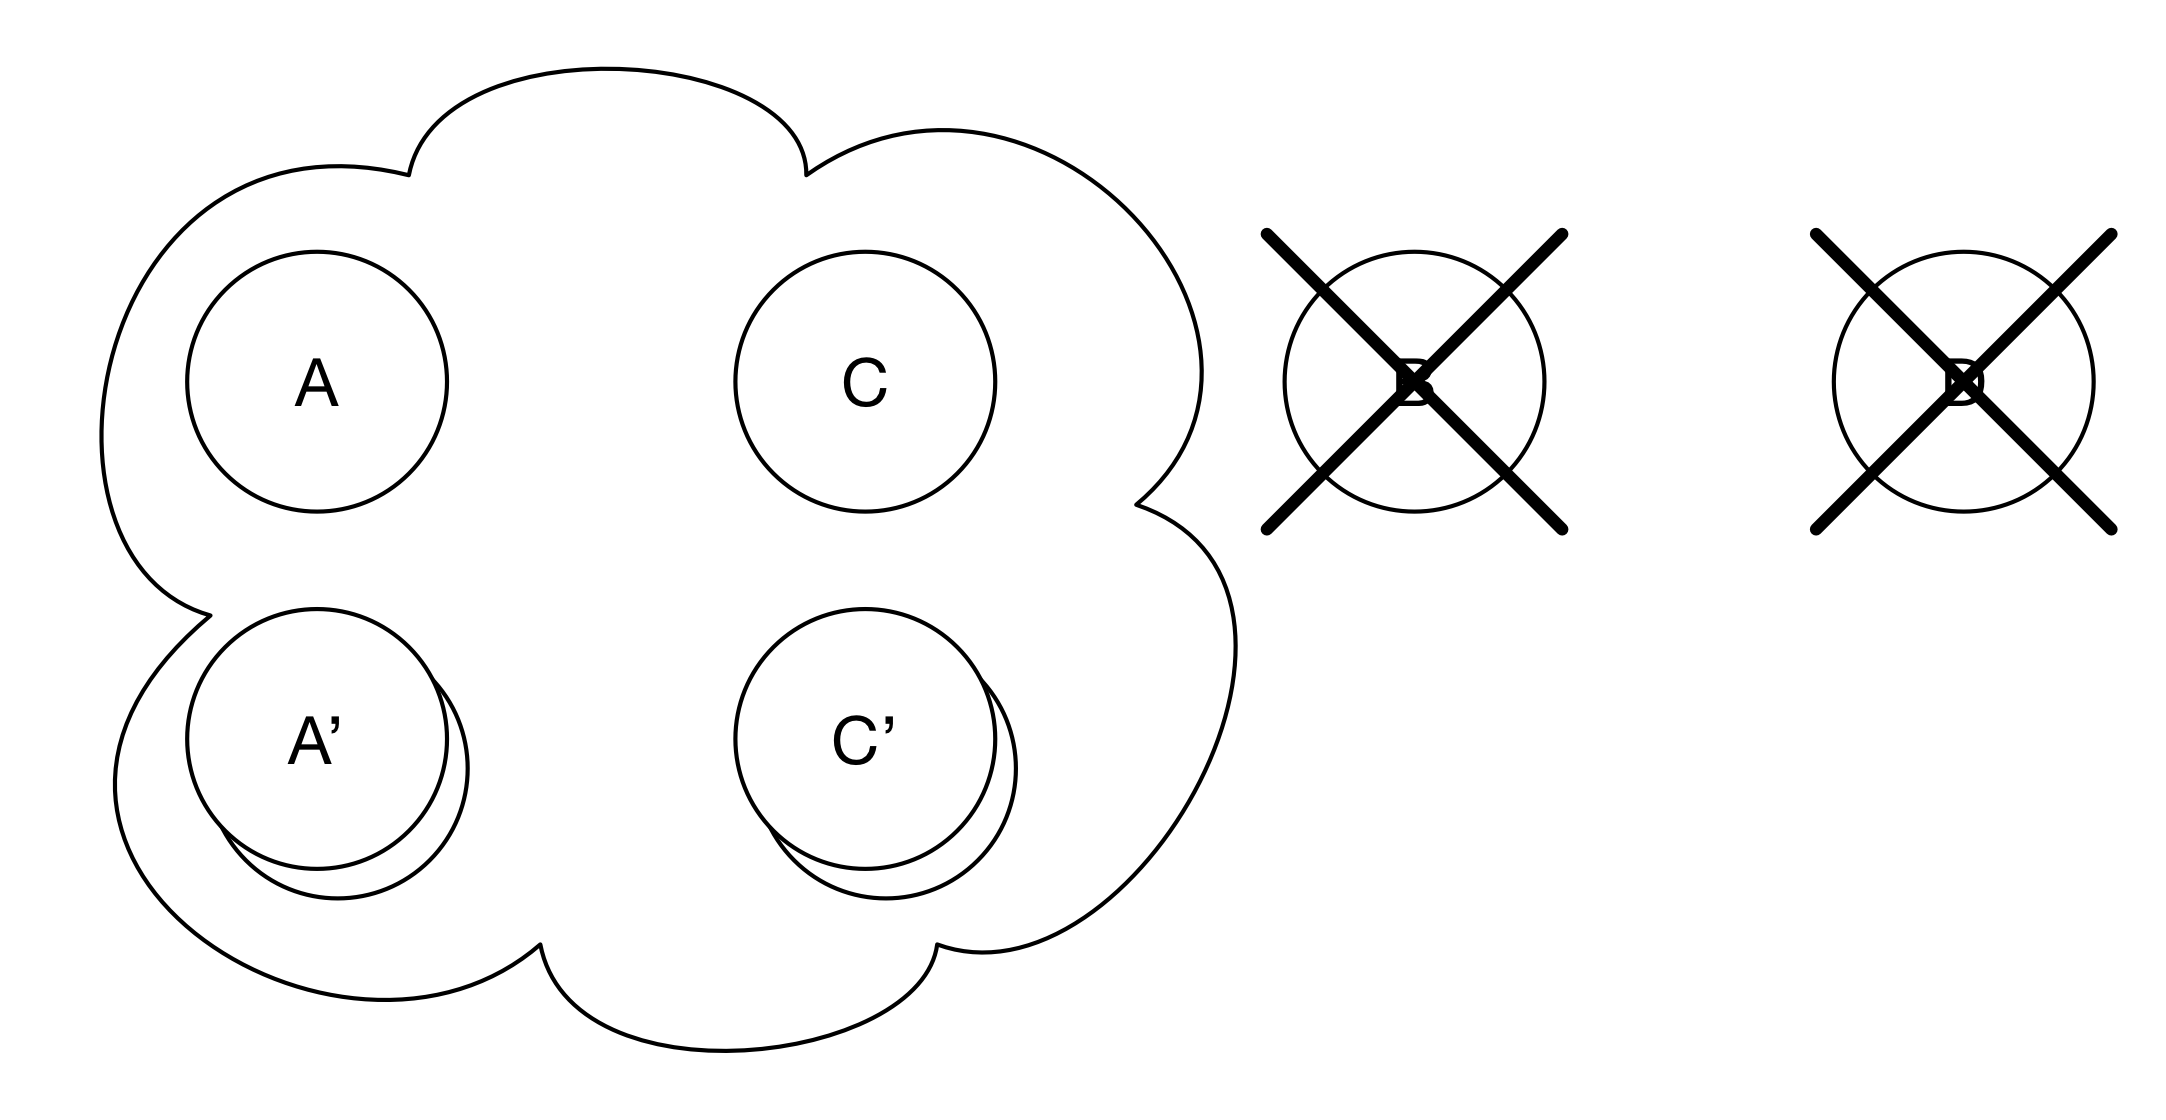
\includegraphics[width=7cm,keepaspectratio]{ri-model-sequence+location.png}
	\end{center}
\end{figure}

With the fine-grained location data available, the application is \emph{expecting} to see a movement that precedes exercises A or C. We call this movement the \emph{setup movement}. The setup movement classifier is a multi-layer perceptron, which takes \SI{1}\second of sensor input and produces probabilities classes that represent the setup movement for groups of exercises. The architecture of the MLP is driven by the sensor data as its inputs; for example, accelerometer-only MLP has 150 inputs (50 samples of the acceleration vector), the subsequent layer has 45 rectifier units, then 40 rectifier units, ending up with 32 softmax units, where 32 is the number of recognised setup movements. The architecture of the MLP for a fully-wired human has 1200 inputs, 250 rectifier units, 100 rectifier units, ending up with 32 softmax units. It is important to measure and optimise the power requirements for the computation; on iOS, we took advantage of the vDSP and veclib frameworks, which offer optimised vector operations. The MLP classes are not the exercises themselves, but the setup movements; one setup movement can map to multiple exercises. To provide accurate prediction of the exercise about to be started, the mobile application takes into account the expected exercise (given the user's typical behaviour), and the fine-grained location data. The performance of the exercise prediction for accelerometer on the user's wrist is shown in \autoref{tbl:setup-movement-performance-accelerometer}; the performance of the exercise prediction rises significantly in fully-wired human (viz \autoref{tbl:setup-movement-performance-all}).

\begin{table}[h]
\caption{Exercise prediction performance (accelerometer)}
\label{tbl:setup-movement-performance-accelerometer}
\begin{center}
\begin{tabular}{|l||m{1cm}|m{1cm}|m{1cm}|m{1cm}|}
\hline            			& Accuracy & Precision & Recall & F1 \\
\hline No context 			& !!       & !!        & !!     & !! \\
\hline Behaviour  			& !!       & !!        & !!     & !! \\ 
\hline Behaviour + Location & !!       & !!        & !!     & !! \\
\hline
\end{tabular}
\end{center}
\end{table}

\begin{table}[h]
\caption{Exercise prediction performance (all sensors)}
\label{tbl:setup-movement-performance-all}
\begin{center}
\begin{tabular}{|l||m{1cm}|m{1cm}|m{1cm}|m{1cm}|}
\hline            			& Accuracy & Precision & Recall & F1 \\
\hline No context 			& !!       & !!        & !!     & !! \\
\hline Behaviour  			& !!       & !!        & !!     & !! \\ 
\hline Behaviour + Location & !!       & !!        & !!     & !! \\
\hline
\end{tabular}
\end{center}
\end{table}

\begin{figure}[hb]
	\begin{center}
		\caption{Exercise sequence model}
		\label{fig:model-sss}
		%\includegraphics[width=7cm,keepaspectratio]{fully-wired.svg}
	\end{center}
\end{figure}


If the user only wears an accelerometer on his or her wrist, then the setup movement for barbell bench press is the same as the setup movement for dumbbell bench press. In 94 \% of our test user base of 451, the next exercise prediction refined by the fine-grained location eliminated ambiguity of setup movement detection in all their exercises. \autoref{fig:model-sequence+setup} shows the final decision state of the mobile application.

\begin{figure}[hb]
	\begin{center}
		\caption{Exercise sequence model}
		\label{fig:model-sequence+setup}
		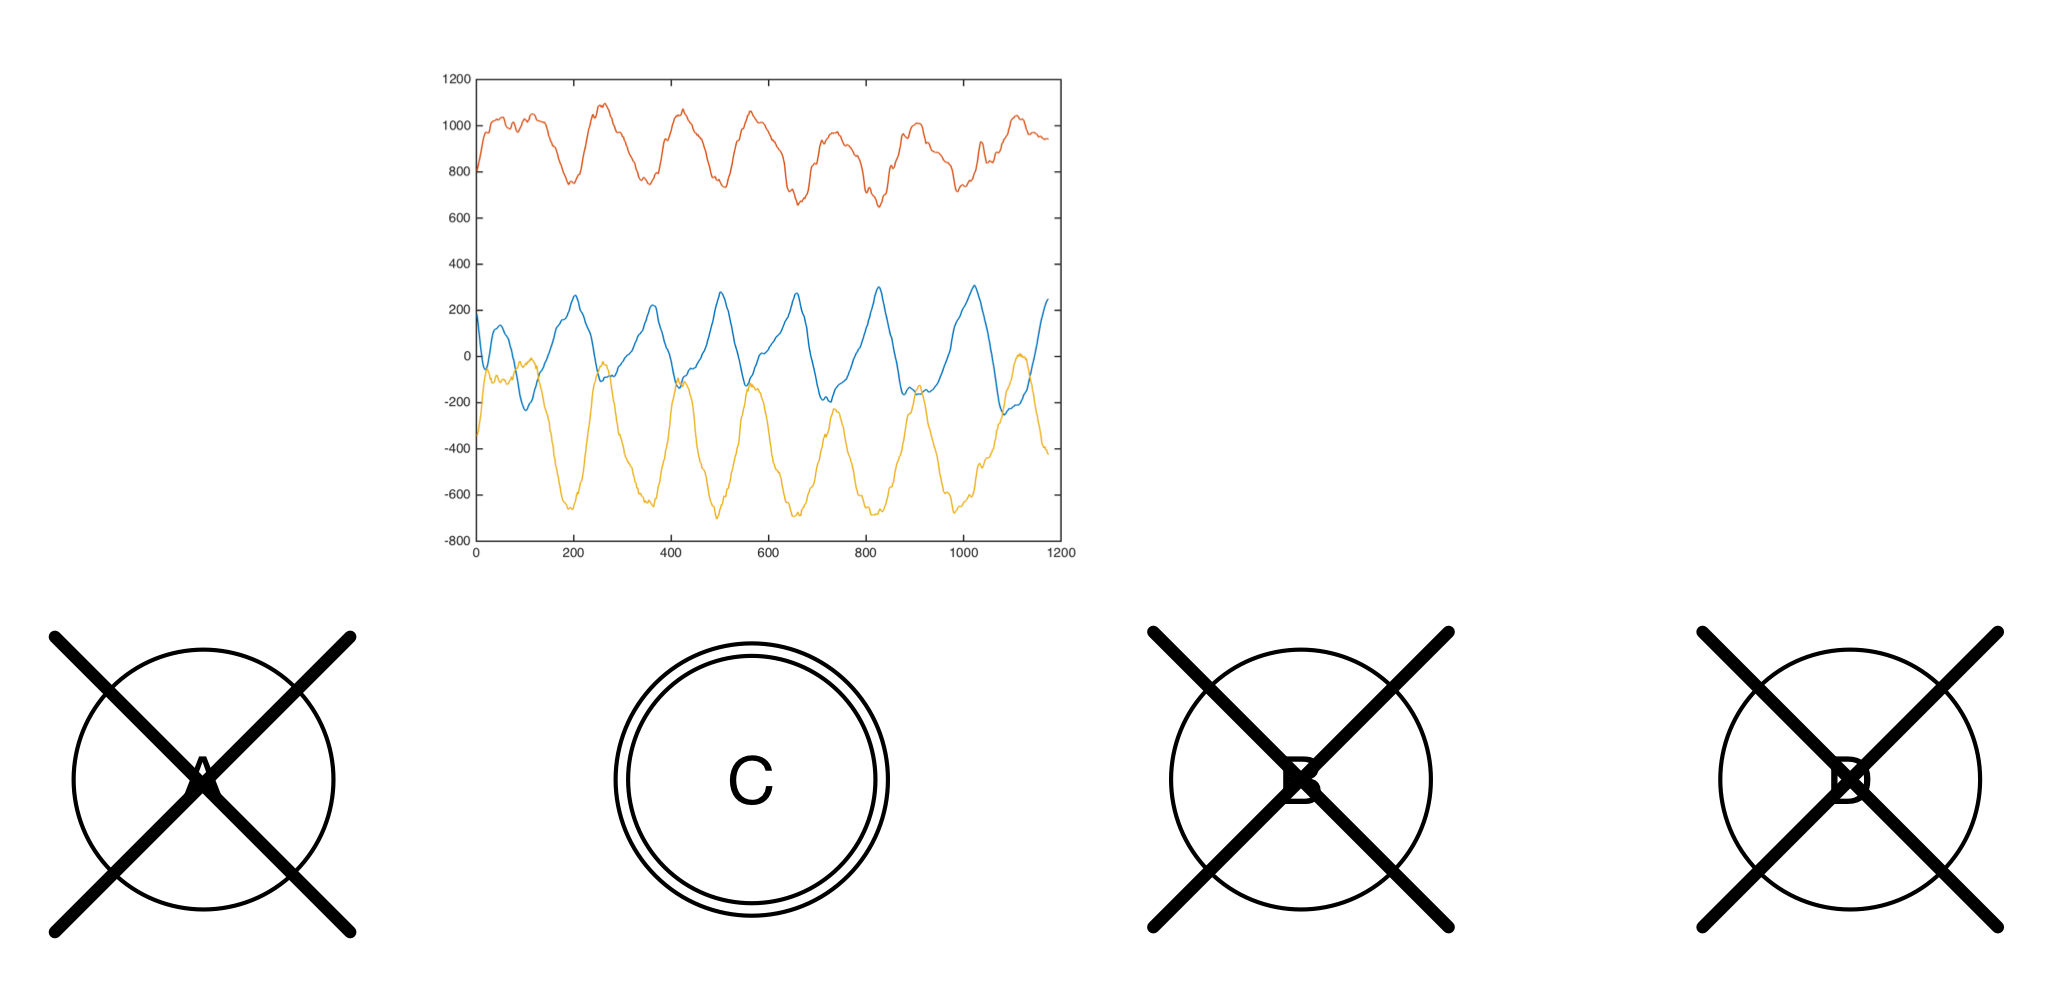
\includegraphics[width=7cm,keepaspectratio]{ri-model-sequence+setup.png}
	\end{center}
\end{figure}

\section{Summary}

TODO

\addtolength{\textheight}{-12cm}  % This command serves to balance the column lengths
                                  % on the last page of the document manually. It shortens
                                  % the textheight of the last page by a suitable amount.
                                  % This command does not take effect until the next page
                                  % so it should come on the page before the last. Make
                                  % sure that you do not shorten the textheight too much.

\begin{thebibliography}{99}

\bibitem{markov-chain-exercise} F. Oo, Q. Uux. Bar. 2016.
\bibitem{akka} Akka.
\bibitem{cqrs-es} CQRS/ES.
\bibitem{apache-cassandra} Apache Cassandra.
\bibitem{apache-spark} Apache Spark.
\bibitem{ibeacon} iBeacon.

\end{thebibliography}


\end{document}
